We investigate how incorporating local topological priors into operand selection affects training dynamics and generalization. Inspired by the locality structure of small-world networks~\cite{watts1998collective}, we initialize each operand selector (\texttt{os1}, \texttt{os2}) to prefer inputs that are spatially adjacent. Specifically, the $i$-th output of \texttt{os1} is initialized to select around input index $i$, while \texttt{os2} is initialized around $i+1$, using a circular Gaussian kernel. No long-range connectivity is imposed; such dependencies must emerge via learning.

We compare this inductive bias (\textit{local init}) with standard dense initialization (\textit{no init}) using OSLGN models with depth 4 and width 512 on MNIST. All other configurations (loss, optimizer, batch size) are held constant.

\paragraph{Generalization.}
As shown in Figure~\ref{fig:smallworld_acc}, the model with local operand initialization achieves higher validation accuracy (39.9\%) compared to standard initialization (34.9\%), despite having lower training accuracy. This suggests that early locality constraints serve as a useful regularizer for symbolic composition.

\paragraph{Gradient Dynamics.}
We further observe that local init results in lower and more stable layer-wise gradient norms (Figure~\ref{fig:smallworld_gradnorm}). This implies that operand selection in the early training phase is smoother and more modular, avoiding large gradient spikes often caused by arbitrary operand mixing.

\paragraph{Learned Distant Connection.}
Although no explicit small-world graph is instantiated, our design encourages a functional small-world effect: high local clustering (via neighborhood initialization) and potential for long-range connections (via training). This stands in contrast to graph-based small-world CNNs~\cite{javaheripi2019swnet}, where topology is hard-coded rather than learned.
The full code used to reproduce these experiments is available at: \footnote{\url{https://colab.research.google.com/drive/1iJpgwW6_7oRRcbllWPLOIW9eeZ0Hcwce?usp=sharing}}

\begin{figure}[H]
    \centering
    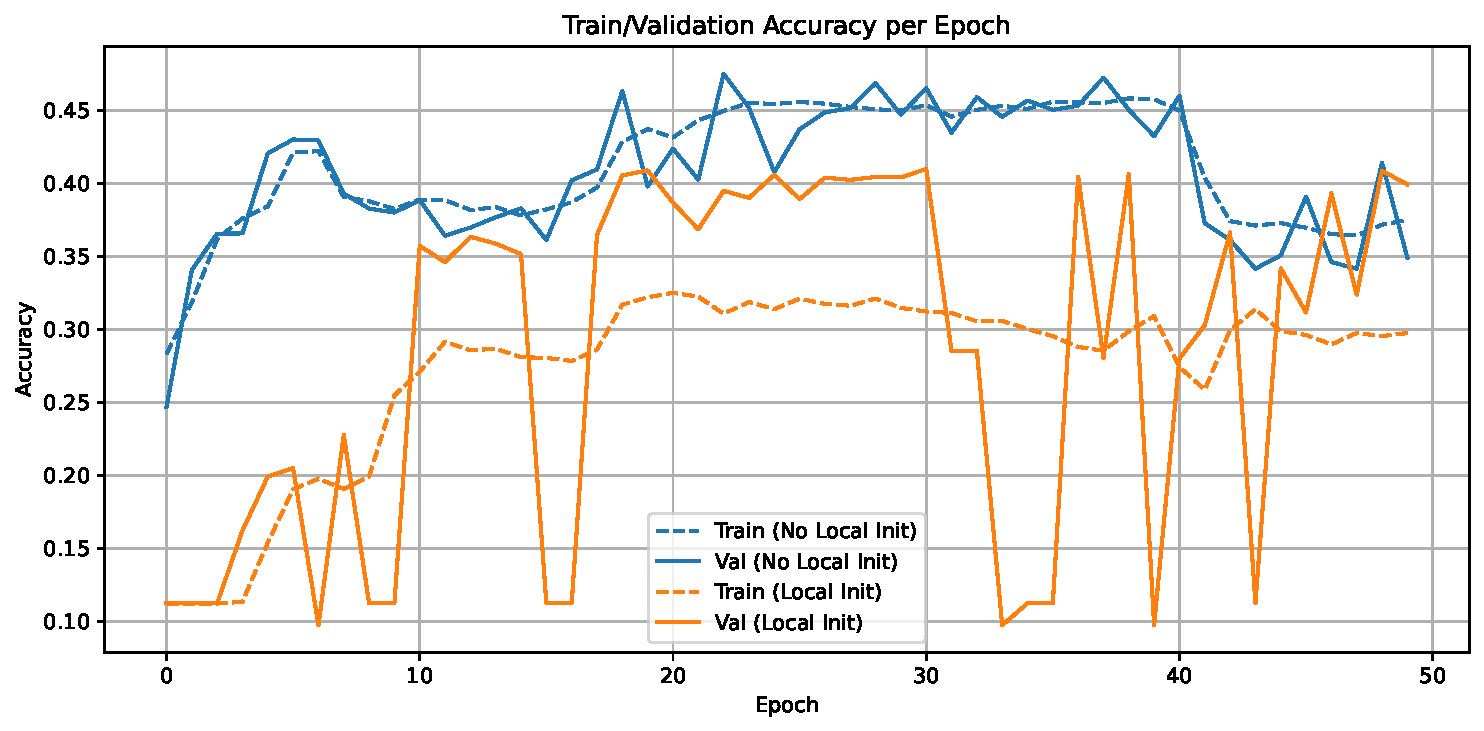
\includegraphics[width=0.45\textwidth]{figures/small_world/accuracy.pdf}
    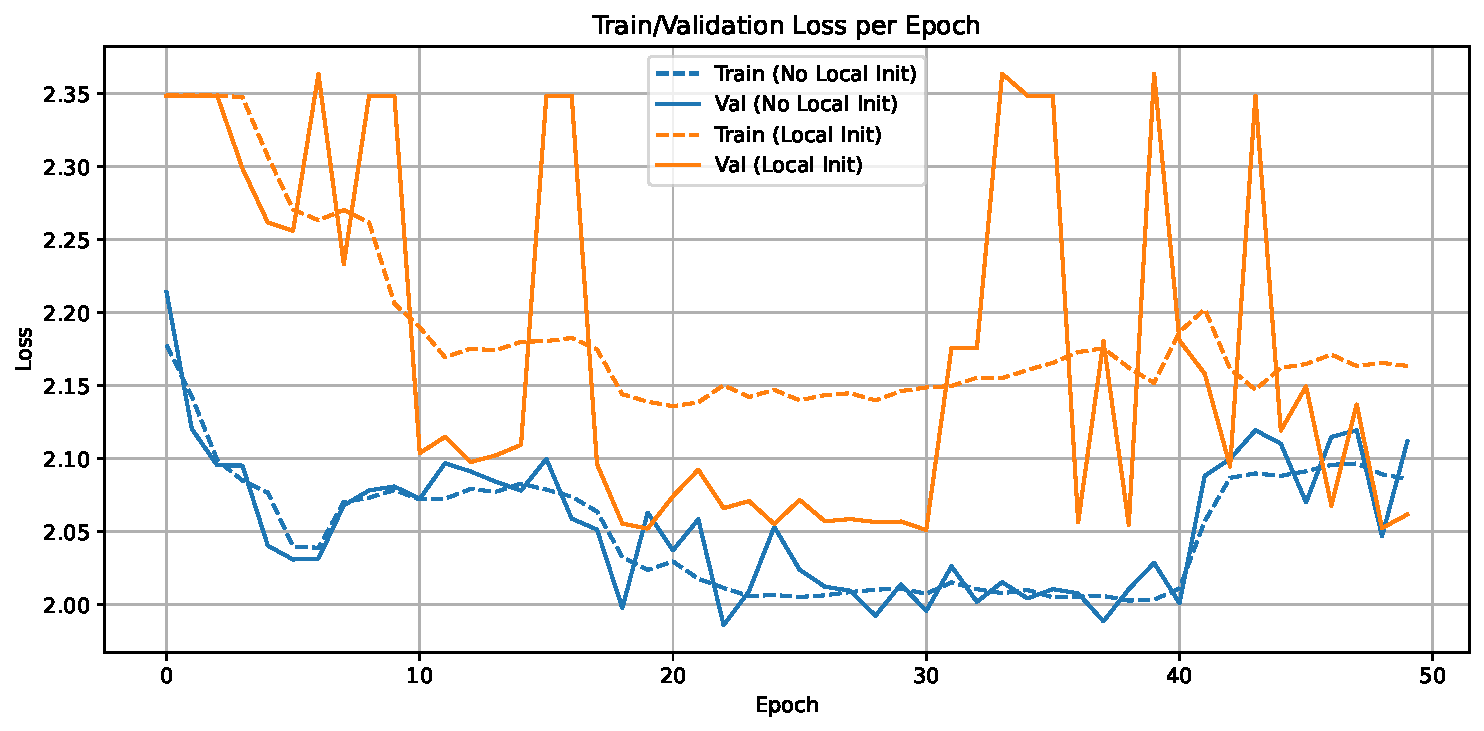
\includegraphics[width=0.45\textwidth]{figures/small_world/loss.pdf}
    \caption{Training and validation accuracy/loss over epochs for OSLGN with and without local operand initialization. Local init generalizes better.}
    \label{fig:smallworld_acc}
\end{figure}

\begin{figure}[H]
    \centering
    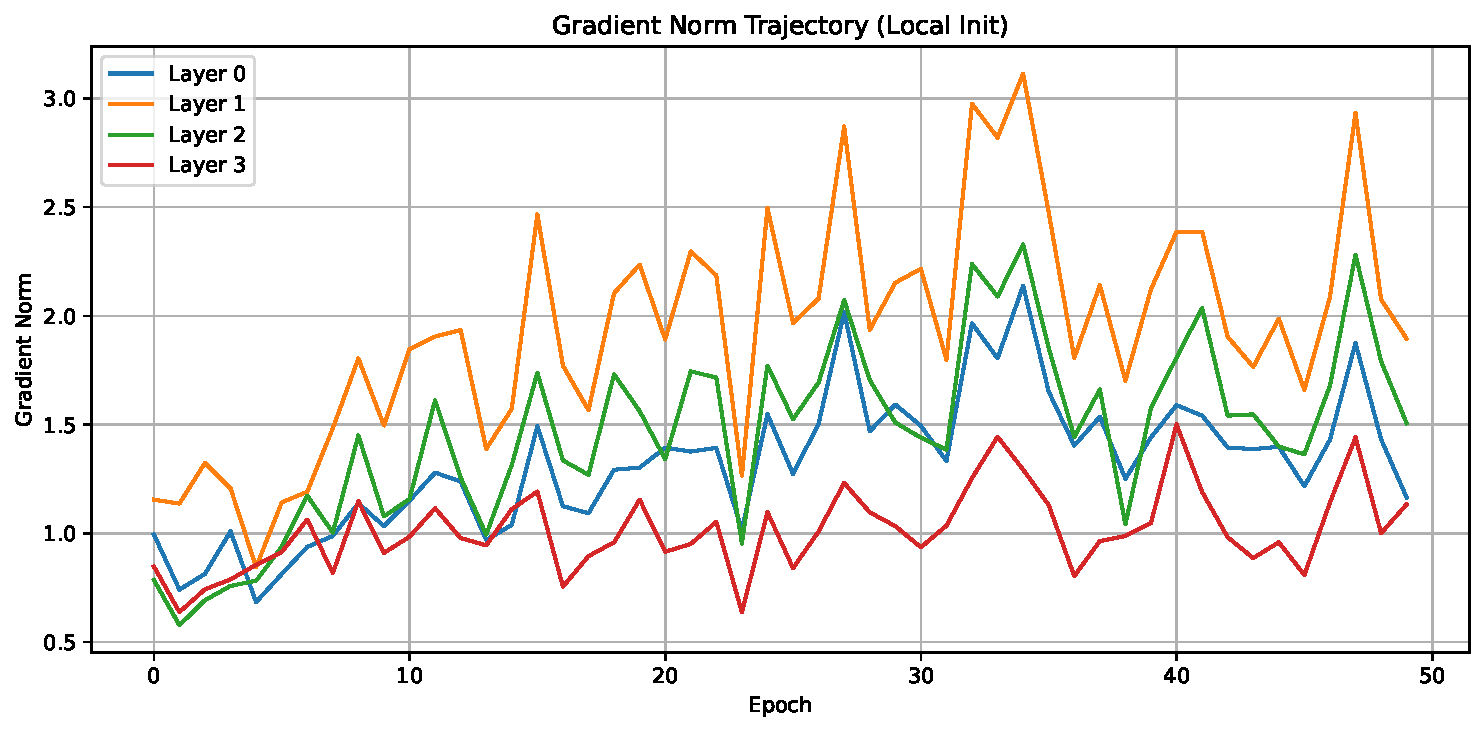
\includegraphics[width=0.85\textwidth]{figures/small_world/gradnorm_lineplot_localinit_on.pdf} \\
    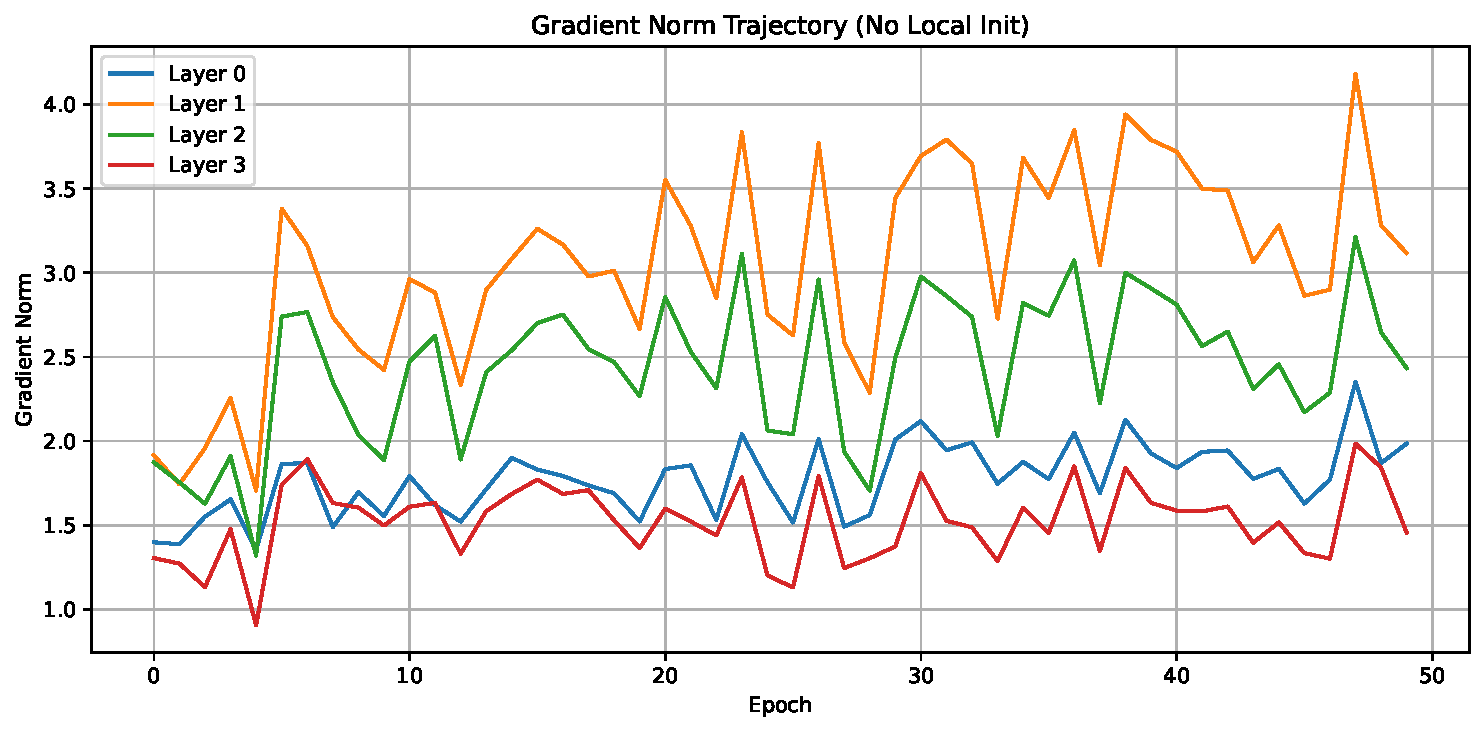
\includegraphics[width=0.85\textwidth]{figures/small_world/gradnorm_lineplot_localinit_off.pdf}
    \caption{Layer-wise gradient norm trajectories with (top) and without (bottom) local operand initialization. Local init results in smoother gradient flow.}
    \label{fig:smallworld_gradnorm}
\end{figure}

